
  \documentclass{beamer}
  \beamertemplatenavigationsymbolsempty
  \setbeamertemplate{footline}[frame number] 
  \setbeamercolor{page number in head/foot}{fg=gray} 
  \usepackage[swedish]{babel}
  \usepackage[utf8]{inputenc}
  \usepackage[T1]{fontenc}
  \usepackage{tgheros, beramono}
  \usepackage{fancyvrb}
  \usepackage{xcolor}
  \definecolor{mygreen}{rgb}{0,0.4,0}
  \definecolor{mylinkcolor}{rgb}{0,0.1,0.5}
  \definecolor{myemphcolor}{rgb}{0,0.4,0.1}
  \definecolor{myalertcolor}{rgb}{0.4,0.1,0}
  \definecolor{eclipsepurple}{rgb}{0.5,0,0.25}
  \definecolor{eclipseblue}{rgb}{0.16,0,1.0}
  \definecolor{eclipsegreen}{rgb}{0,0.5,0}
  \usepackage{listings}

  %%% lingstings specifics:

  \lstdefinelanguage{Scala}{
    morekeywords={abstract,case,catch,class,def,%
      do,else,enum,export,extends,false,final,finally,%
      for,given,if,implicit,import,lazy,match,%
      new,null,object,override,package,%
      private,protected,return,sealed,%
      super,then,throw,trait,true,try,%
      type,val,var,while,with,yield,%
      as, derives, end, extension, infix, inline, opaque, open, transparent, using}, % soft keywords
    otherkeywords={=>,<-,<:,>:,@,=>>,?=>},
    sensitive=true,
    morecomment=[l]{//},
    morecomment=[n]{/*}{*/},
    morestring=[b]",
    morestring=[b]',
    morestring=[b]"""
  }

  \lstset{
      language=Scala,
      tabsize=2,
      basicstyle=\ttfamily,
      keywordstyle=\bfseries\color{eclipsepurple},
      commentstyle=\color{mygreen},
      numberstyle={\footnotesize},
      numbers=none,
      %backgroundcolor=\color{gray!15},
      frame=none, %single,
      rulecolor=\color{black!25},
      %title={\footnotesize\lstname},
      breaklines=false,
      breakatwhitespace=false,
      framextopmargin=2pt,
      framexbottommargin=2pt,
      showstringspaces=false,
      columns=fullflexible,keepspaces
  }

  \lstset{literate=%
  {Å}{{\AA}}1
  {Ä}{{\"A}}1
  {Ö}{{\"O}}1
  {Ü}{{\"U}}1
  {ß}{{\ss}}1
  {ü}{{\"u}}1
  {å}{{\aa}}1
  {ä}{{\"a}}1
  {ö}{{\"o}}1
  {æ}{{\ae}}1
  {ø}{{\o}}1
  {Æ}{{\AE}}1
  {Ø}{{\O}}1
  {`}{{\`{}}}1
  {─}{{\textemdash}}1
  {└}{{|}}1
  {├}{{|}}1
  {│}{{|}}1
  {♠}{{$\spadesuit$}}1
  {♥}{{$\heartsuit$}}1
  {♣}{{$\clubsuit$}}1
  {♦}{{$\diamondsuit$}}1
  }

  \lstnewenvironment{Scala}[1][]{%
      \lstset{#1}%
  }{}  
    
\author{Björn Regnell}
\title{Introduction to Software\\Requirements Engineering}
\usepackage[yyyymmdd]{datetime}
\renewcommand{\dateseparator}{--}
\date{\footnotesize Updated: \today}
\begin{document}
\maketitle

\begin{frame}[fragile]{About Björn Regnell}
\begin{minipage}[t][1.0\textheight]{0.78\textwidth}
\vspace{0pt}
\begin{itemize}
\item Professor in Software Engineering at the Faculty of Engineering, LTH, Lund University, Sweden.
\item Research areas: 
\begin{itemize}
\item Software Engineering
\item Requirements Engineering 
\item Empirical research methods in Software Engineering 
\end{itemize}
\item Current teaching: 
\begin{itemize}
\item Software Requirements Engineering
\item Introduction to Programming in Scala 
\end{itemize}
\item Homepage: 
\begin{itemize}
\item \url{https://cs.lth.se/bjorn-regnell}
\end{itemize}
\end{itemize}
\end{minipage}%
\hspace*{1em}\begin{minipage}[t][1.0\textheight]{0.22\textwidth}
\vspace{0pt}\hfill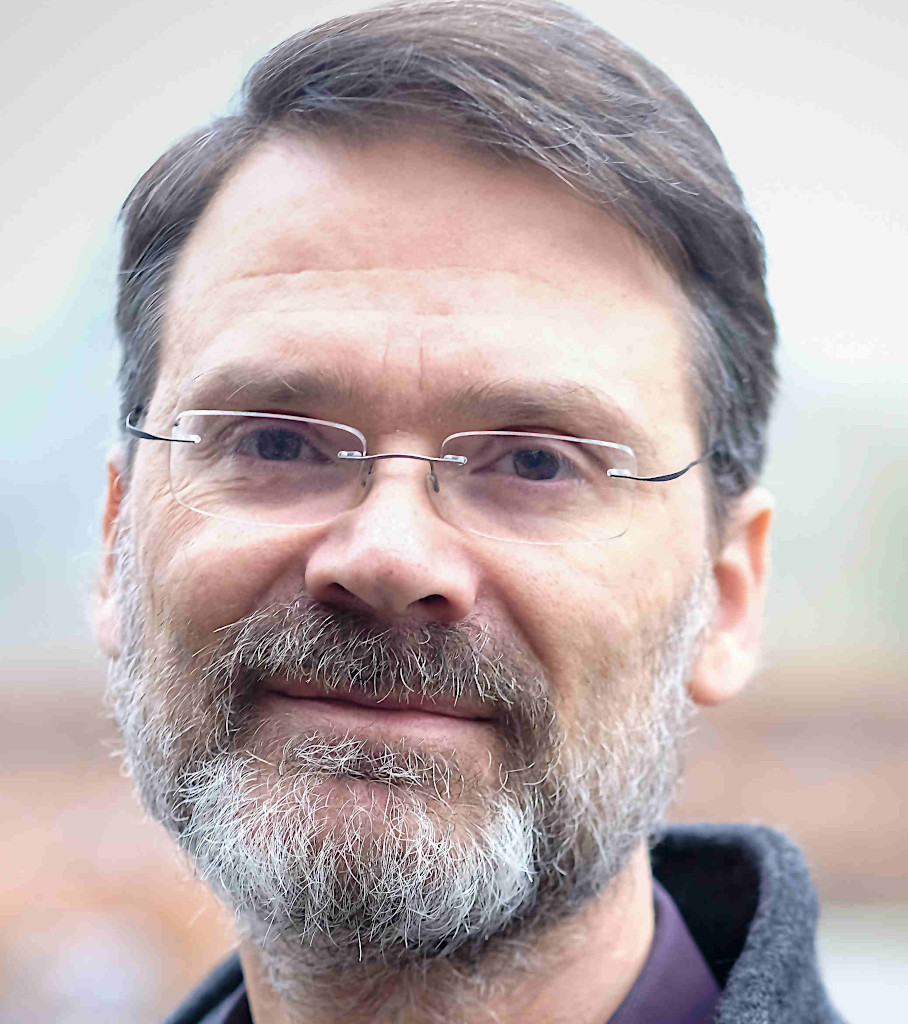
\includegraphics[width=0.9\textwidth]{img/bjorn-regnell}
\end{minipage}%
\end{frame}

\begin{frame}[fragile]{What is Requirements Engineering (RE)?}
\begin{itemize}
\item  Requirements Engineering (RE) is a sub-discipline of Software Engineering (SE) that is focused on the \textit{requirements} of software-intensive systems and their \textit{context}, which includes users and surrounding systems.
\item When you work with anything related to the \textit{decision-making process} of software development and its \emph{underlying intentions} you are doing requirements engineering.
\end{itemize}
\end{frame}

\begin{frame}[fragile]{What is a requirement?}
\begin{itemize}
\item Something needed or wanted.
\item A documented representation of \\something needed or wanted.
\item The word ''requirement'' can have different meanings:
\begin{itemize}
\item ... must, wish, idea, design detail, rationale, ...
\item The most general meaning of ''requirement'':
\item[] \emph{any} kind of information entity used in RE
\end{itemize}
\end{itemize}
\end{frame}

\begin{frame}[fragile]{Activities in Requirements Engineering}
The work you do withing Requirements Engineering is often described in terms of these four activities:
\begin{itemize}
\item \textbf{Elicitation}: learn, invent, agree.
\item \textbf{Specification}: represent, persist, communicate.
\item \textbf{Validation}: check that representations are good enough.
\item \textbf{Selection}: prioritize, decide, plan.
\end{itemize}
\vspace*{1em}
These activities are often conducted \textbf{concurrently} and \textbf{iteratively}, throughout the product life-cycle.
\end{frame}

\begin{frame}[fragile]{The Context of Requirements Engineering}
%\begin{itemize}
%\item 
How to best do RE is \textbf{highly context-dependent}:
\begin{itemize} 
\item \textbf{Stakeholder configuration}: relation customer -- supplier
\\\textit{Type of Customer}: business partner, public authority, private consumer on a market
\\\textit{Type of Supplier}: consultancy, product integrator, subcontractor, open-source contributor in a community
\item \textbf{The funding model}, risk-sharing customer -- supplier:
\\not-for-profit/donation, internal use, share of sales, fixed license fee, service subscription, freemium, ad-based, ... 
\item \textbf{Level of customization}:
\\generic, customized, customer specific
\item \textbf{Hardware integration}:
\\pure software, hardware + software
\item \textbf{Network integration}:
\\stand-alone, connected, distributed
\item \textbf{Delivery model}:
\\one-off, eventually updated, continuous delivery
\end{itemize}
%\end{itemize}
\end{frame}

\begin{frame}[fragile]{Requirements Modelling}
\begin{itemize}
\item Finding the right level of quality of representations:
\begin{itemize}
\item What is good enough for now?
\item When are we ''ready'' with this part of the model?
\end{itemize}
\item Representing related functionality and quality
\item Representing requirements at different levels
\end{itemize}
\end{frame}

\begin{frame}[fragile]{Good enough requirements representations}
What is a good enough requirements model?
\\ \vspace*{0.5em}Examples of quality aspects, achievable to some degree:
\begin{itemize}
\item \textbf{Correctness}: reflect the expected, intended behavior
\item \textbf{Unambiguity}: stakholders have similar interpretation
\item \textbf{Completeness}: most important, relevant aspects included
\item \textbf{Consistency}: no contradictions among requirements
\item \textbf{Conciseness}: suitable level of abstraction and detail 
\item \textbf{Comprehensibility}: understood by stakeholders 
\item \textbf{Verifiability}: possible to check fulfillment 
\item \textbf{Feasibility}: possible to implement, value to justifiable cost 
\item \textbf{Traceability}: can be referred to, can find its origin
\item \textbf{Modifyability}: easy to change, good structure
\item \textbf{Ranked}: includes evaluations of importance and stability
\end{itemize}
\end{frame}

\begin{frame}[fragile]{Requirements on System Functionality}
\begin{itemize}
\item \textbf{Data}: information stored by the system 
\begin{itemize}
\item domain-specific data entities
\item format of input and output data
\item representation of (externally visible) system state
\end{itemize}

\item \textbf{Logic}: the functional relation between input and output 
\begin{itemize}
\item logical behavior, state transitions, computation
\item dynamic relation between input and output
\begin{itemize}
  \item specifying desired output given:
  \item expected and unexpected input
  \item current system state
  \item relevant usage situations
\end{itemize}
\end{itemize}

\end{itemize}
\end{frame}

\begin{frame}[fragile]{Requriements on System Quality}
\begin{itemize}
\item Goodness of implementation of intended functionality 
\begin{itemize}
  \item A level on a sliding scale.
  \item What is good enough?
  \item System-wide or specific to a certain feature?
\end{itemize}
\item Examples of quality aspects:
\begin{itemize}
\item \textbf{Accuracy}: Precisions of data.
\item \textbf{Capacity}: Resources per time unit.
\item \textbf{Performance}: Response time.
\item \textbf{Reliability}: Number of bugs, failure rate.
\item \textbf{Security}: Protect system from damage by malicious users. 
\item \textbf{Safety}: Protect users from being damaged by the system.
\item \textbf{Maintainability}: Easy to fix bugs and adapt the system.
\item \textbf{Usability}: Subjective and objective experience of users:\\ easy learn, supports my tasks, easy to remember, easy to understand, attractive: ''I like it!'' 
\end{itemize}
\end{itemize}
\end{frame}

\begin{frame}[fragile]{Requirements at Different Levels}
\begin{itemize}
\item Levels of Abstraction: the Goal-Design scale 
\item Levels of Detail: amount and richness of information 
\item Levels of Aggregation: grouping and linking 
\item Levels of Formality: automatic checks of syntax and semantics, (partial) proofs of correctness
\end{itemize}
\end{frame}

\begin{frame}[fragile]{Levels of abstraction: The Goal-Design scale}
\begin{itemize}
\item Goal-level: represents the intentions of stakeholders; why? 
\item Domain-level: represents how users collaborate with the system to achieve their goals
\item Product-level: represents the relation between input and expected response; what?
\item Design-level:\\represents upfront decisions on system design, how?\\often based on existing systems and standards, often needs extra validation e.g. prototyping
\end{itemize}
\end{frame}

\begin{frame}[fragile]{Automated support for RE}
\begin{itemize}
\item Databases
\item Support for writing, drawing, recording
\item Traceability 
\item Search and summarize
\item Adapt views to specific stakeholders
\item AI for RE
\begin{itemize}
\item AI support to elicit, specify, validate, select 
\item Meta-level RE:\\RE for AI for RE
\end{itemize}
\end{itemize}
\end{frame}

\begin{frame}[fragile]{Methods of Representation}
Examples of requirements representations:
\begin{itemize}
\item Context diagram
\item Goal models: stakeholders, goals+relations (helps, hurts)
\item Data Models: E/R-diagrams, Data dictionaries
\item Feature Models (in text or pictures):\\why, what: function+data, examples of how,\\expected quality,\\links to other features and model
\item Dynamic Models: 
\begin{itemize}
\item Scenario-based models:\\narratives, user stories, task models, use case models
\item State-transition models: state diagrams, transition matrices
\item Test Cases: acceptance tests, system tests, unit tests
\item User interface models: mockups, GUI Designs
\end{itemize}
\end{itemize}
\end{frame}

\begin{frame}[fragile]{Representing the state of a feature}
Example of how to represent the state of a feature:
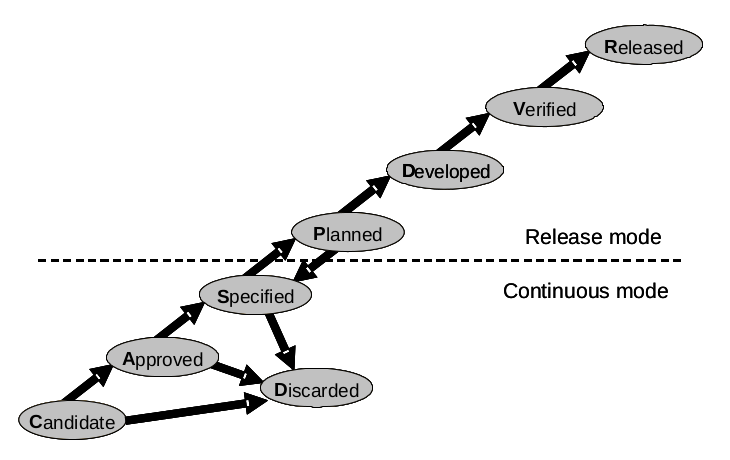
\includegraphics[width=0.9\textwidth]{img/ladder}
''Feature release ladder''
\end{frame}



    
\end{document}

